%% technisch.tex
%% $Id: technisch.tex 61 2012-05-03 13:58:03Z bless $
%%

\chapter{Technische Speicherung}
\label{ch:Technische Speicherung}
%% ==============================  

	%% ==============================
    \section{Elektronische Speicherung}
    %% ==============================
    \label{ch:Technisch:sec:Elektronische Speicherung}
    %% ==============================
	
	Alle Speichermedien die Daten auf Basis von elektronischen Bauelementen speichern sind unter dem Begriff elektronische Speicher zusammengefasst. Heutzutage werden die integrierten Schaltkreise, die zur elektrischen Speicherung notwendig sind fast nur noch mit Silizium realisert. Die einzelnen k"onnen beliebig angesprochen werden, es ist also keine weitere Teilung des Speichers in Sequenzen notwendig. Weiter unterschieden werden elektronische Speichermedien in fl"uchtige Speicher, permanente Speicher und semi-permanente Speicher.
	
        \subsection{Fl"uchtig}
        %% ==============================
        \label{ch:Technisch:sec:Elektronische Speicherung:sub:Fl"uchtig}
        %% ==============================
        
            Ein fl"uchtiger Speicher kann seine Information nur behalten, wenn er an einem Strom liegt, andernfalls verliert er diese Informationen.
				
				\subsubsection{DRAM}
				%% ==============================
				\label{ch:Technisch:sec:Elektronische Speicherung:sub:Fl"uchtig:subsub:DRAM}
				%% ==============================
				
					Beim \glqq Dynamic Random Access Memory\grqq{} handelt es sich um Speicherbausteine, die nach dem Abschalten der angelegten Spannungsversorgung oder zu späten Wiederauffrischung ihren Dateninhalt auf den Speicherzellen verlieren. Der volatile\footnote{fl"uchtig} Speicher wird haupts"achlich in Computern als Arbeitspeicher eingesetzt, man findet ihn aber auch beispielsweise in Druckern oder in Videospielkonsolen.
					\\
					Technisch gesehen speichert ein Kondensator die Daten, also Einsen und Nullen in dem er entweder geladen oder entladen ist. Ein Schalttransistor beschreibt oder liest den Inhalt dann aus.
				
				\subsubsection{SRAM}
				%% ==============================
				\label{ch:Technisch:sec:Elektronische Speicherung:sub:Fl"uchtig:subsub:SRAM}
				%% ==============================
				
					Der \glqq Static Random Access Memory\grqq{} ist wie der DRAM ebenfalls ein Halbleiterspeicher, der volatil ist. Dauerhaft kann er Daten nur speichern, wenn er mit Strom versorgt wird. Der Unterschied zum DRAM ist dabei, dass der Inhalt nicht wiederaufgefrischt werden muss, da SRAM mit Flipflops realisiert wird. Ein Flipflop oder auch bistabile Kippstufe kann zwei Zust"ande(Eins oder Null) einnehmen und "uber lange Zeit speichern, allerdings ist die Speicherzelle des SRAM im Vergleich zum DRAM relativ gro"s.
					\\
					Anwendung findet SRAM in Prozessoren als \textit{Cache} oder in Bereichen bei denen der Dateninhalt "uber l"angere Zeit gespeichert werden soll wie beim CMOS-RAM zur Erhaltung von BIOS-Einstellung\footnote{Basic Input Output System} in PCs und Laptops. Zur Aufrechterhaltung der Stromversorung gen"ugt meist eine kleine Pufferbatterie.
					
        
        \subsection{Permanent}
        %% ==============================
        \label{ch:Technisch:sec:Elektronische Speicherung:sub:Permanent}
        %% ==============================
        
            Permanenter Speicher beh"alt seine Daten, die einmal in ihm gespeichert oder verdrahtet wurde. Er kann dann nicht mehr ver"andert werden.
			
				\subsubsection{ROM}
				%% ==============================
				\label{ch:Technisch:sec:Elektronische Speicherung:sub:Fl"uchtig:subsub:ROM}
				%% ==============================
				
					Ein typisches Beispiel f"uer permanten Speicher ist der \glqq Read Only Memory\grqq{} – zu Deutsch \textit{Festwertspeicher} oder \textit{Nur-Lese-Speicher}. ROM kann nur einmal beschrieben werden, dann lassen sich die darauf geschriebenen Daten nicht mehr, nur sehr langsam oder schwer ver"andern. 
					\\
					Die Hauptanwendung ist somit die Verbreitung und Speicherung von Firmware\footnote{Software die spezifisch an Hardware angepasst ist, "ahnlich einem Betriebsystem, aber selten ein Update braucht}. Auch das BIOS eines PCs ist auf einem ROM gespeichert.
					\\
					Klassische Masken-ROM werden so genannt, weil urspr"unglich ROM in der Herstellung mit einer Art Filmnegativ – der \glqq Maske\grqq{} direkt auf den Chip aufbelichtet wird. Das Verfahren ist aber nur in Massenproduktion "okonomisch Sinnvoll, weshalb bald Speicherbausteine entwickelt wurden, die auch nach der Fertigung noch mit Daten bef"ullt werden konnten.
				
				\subsubsection{PROM}
				%% ==============================
				\label{ch:Technisch:sec:Elektronische Speicherung:sub:Fl"uchtig:subsub:PROM}
				%% ==============================
				
					Einer dieser neu entwickelten Speicherbausteine ist das \glqq Programmable Read Only Memory\grqq{}. Diese lassen sich nach der Fertigung genau einmal Programmieren und behalten dann ihren Zustand. Anfangs enthalten alle Speicherzellen eine \glqq 1\grqq{}, einzelne Speicherzellen k"onnen dann sp"ater in eine \glqq0\grqq{} gewandelt werden.
					\\
					Praktisch werden PROMs heute nicht mehr verwendet. 
            
        \subsection{Semi-permanent}
        %% ==============================
        \label{ch:Technisch:sec:Elektronische Speicherung:sub:Semi-permanent}
        %% ==============================
        
            Von semi-permanenten Speichern spricht man, wenn die Daten permanent gespeichert werden, aber im Gegensatz zum permanenten Speicher auch wieder ver"andert werden k"onnen. 
			
				\subsubsection{EPROM}
				%% ==============================
				\label{ch:Technisch:sec:Elektronische Speicherung:sub:Fl"uchtig:subsub:EPROM}
				%% ==============================
					
					Bei der EPROM-Technologie handelt es sich um die Weiterentwicklung von ROM. EPROM steht f"ur \glqq Erasable Programmable Read Only Memory\grqq{} und ist ROM, der aber auch wieder gel"oscht(und damit ver"andert) werden kann. Damit man aber EPROMs programmieren kann, bedarf es spezieller Progammierger"ate – dem \glqq EPROM-Brenner\grqq{}. Mit UV-Licht kann der Speicher dann wieder gel"oscht werden.
					\\
					Weiterhin gibt es noch elektronisch l"oschbaren Speicher EEPROM(\glqq Electrical Erasable Read Only Memory\grqq{}), welches mit Flash-EEPROM EPROM verdr"angt hat.
				
				\subsubsection{Flash-EEPROM}
				%% ==============================
				\label{ch:Technisch:sec:Elektronische Speicherung:sub:Fl"uchtig:subsub:Flash-EEPROM}
				%% ==============================
				
					Dieser elektronisch l"oschbare ROM EEPROM(\glqq Electrical Erasable Read Only Memory\grqq{}) hat den entscheidenen Vorteil, dass er kein spezielles Verfahren braucht um neu beschrieben zu werden; gleichzeitig beh"alt er auf ihm gespeicherte Daten auch ohne eine Spannung aufrecht erhalten zu m"ussen. Ein im Alltag sehr bekannter Begleiter dieses Speicherverfahrens ist der USB-Stick. 
					\\
					Durch seine kompakten Ma"se ist er sehr portabel und die mittlerweile g"angigen Speichergr"o"sen reichen von 2 Gigabyte bis zu 256 GB. Er l"asst sich an jeden USB-Host anschlie"sen, Daten lassen sich so einfach austauschen. 
					\\
					Da die Entwicklung der Flash Speicher erst sp"at begonnen hat, lassen sich heute noch nicht die Speichergr"o"sen von handels"ublichen Festplatten erreichen, doch daf"ur sind sie stromsparender und deutlich praktischer.
				
				\subsubsection{SSD}
				%% ==============================
				\label{ch:Technisch:sec:Elektronische Speicherung:sub:Fl"uchtig:subsub:SSD}
				%% ==============================
				
				%Obwohl die SSD nicht ganz mit der Pyramide vereinbar ist, geh"ort sie trotzdem in die obere Sektion%%eventuell in die einleitung schreiben??
				Die Solid State Drive(SSD) ist ein nichtfl"uchtiger und auf Flash-Technologie basierter Speicher. Er hat keine mechanisch beweglichen Teile mehr wie bei der konventionellen Festplatte. Dadurch vebraucht sie weniger Strom und die Zugriffszeiten sind enorm hoch. H"aufig werden SSDs im 2,5$"$ Format verkauft, sie sind allerdings nicht an die Normen f"ur optische oder magnetische Speicherplatten gebunden und sind daher z.B. auch als PCI-Steckkarte aufzufinden. Die nachfolgende Abbildung zeigt das Innenleben einer SSD im 2,5$"$ Format halbtransparent.
				\begin{figure}[ht]
				\centering
				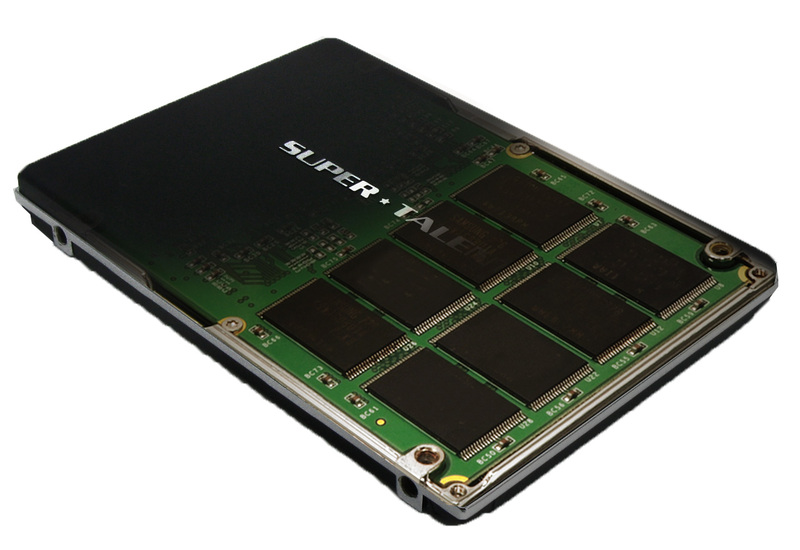
\includegraphics[width=0.7\textwidth]{images/ssd} 
				\caption[SSD innenleben \cite{fig:ssd}]{SSD innenleben}
				\label{fig:ssd}
				\end{figure}
				\\
				Durch die immer weiter sinkenden Preise pro Gigabyte und die unumst"o"slichen Vorteile ist eine dauerfristige Abl"osung von magnetischen Fesplatten durch Solid State Drives zu sehen.
				
				
%% ==============================%% ==============================%% ==============================%% ==============================   		
			
			
			
    %% ==============================
    \section{Magnetische Speicherung}
    %% ==============================
    \label{ch:Technisch:sec:Magnetische Speicherung}
    %% ==============================
    
    Magnetische Speichermedien behalten ihre Informationen, in dem mit Hilfe eines Lese-Schreib-Kopfes Daten auf magnetisierbares Material gebracht werden. Unterschieden wird dann jeweils weiter in nicht rotierende und rotierende Speichermedien. Die nicht rotierenden Speichermedien werden weiter in digitale und analoge Medien unterteilt. Zum ersteren geh"oren Magnetstreifen oder Magnetband. Ein analoges nicht rotierendes Speichermedium ist das Ton- oder Videoband. Die bekannten Festplatten werden zu rotierenden Speichermedien gez"ahlt und sind heute der weit verbreiteste Massenspeicher.

        \subsection{Festplatte}
        %% ==============================
        \label{ch:Technisch:sec:Magnetische Speicherung:sub:Festplatte}
        %% ==============================
        
            Die Festplatte oder das Festplattenlaufwerk speichert Informationen, in dem sie Daten auf die Oberfl"ache einer rotierenden Scheibe schreibt. Die Scheiben sind genau "ubereinander gelagert und drehen sich zur selben Zeit. Die hartmagnetische Beschichtung an der Plattenoberfl"ache wird dann mit den Lese-Schreib-Kopf entweder gelesen oder beschrieben. Auf die Daten kann wahlfrei zugegriffen werden und auch nach dem Ausschalten bleiben die Daten durch Remanenz\footnote{Remanenz ist die zur"uckbleibende Magnetisierung eines magnetischen K"orpers} erhalten. W"ahrend die erste Fesplatte noch eine Tonne wog und nur eine Kapazit"at von 5 Megabyte hatte, haben heutige Festplatten eine Gr"o"se von bis zu 4 Terabyte. Im Gegensatz zu einer SSD k"onnen Festplatten nahezu beliebig oft gel"oscht und neu beschrieben werden.
			\\
			Die Abbildung \ref{fig:hdd} zeigt den schematischen Aufbau einer Festplatte.
			\begin{figure}[ht]
				\centering
				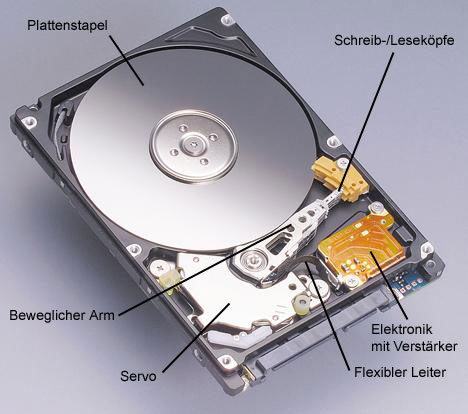
\includegraphics[width=0.6\textwidth]{images/hdd} 
				\caption[Festplattenaufbau \cite{fig:hdd}]{Festplattenaufbau}
				\label{fig:hdd}
				\end{figure}
            \\
            Das Anschlie"sen an einen PC erfolgt mittlerweile entweder intern "uber den Serial ATA-Anschluss oder extern "uber USB\footnote{Universal Serial Bus}, Firewire, Thunderbolt oder eSATA. 
    
    
    %% ==============================
    \section{Optische Speicherung}
    %% ==============================
    \label{ch:Technisch:sec:Optische Speicherung}
    %% ==============================
    
        Das optische Speichermedium erh"alt die Daten entweder mechanisch in einem Presswerk(meist kommerziell hergestellte Disks) oder "uber einen Laser(meist private so gennante \glqq gebrannte\grqq{} Disks) in Form von Erh"ohungen(Pits) und Vertiefungen(Lands) auf eine Scheibe. Meistens trifft man bei optischen Speichermedien auf die CD, der DVD oder der Blu-ray Disc. Diese unterscheiden sich in ihrer Speicherkapazit"at, jedoch nicht in ihrer physikalischen Gr"o"se – 8$"$ Durchmesser.
        \\
		Die Funktionsweise ist nochmals in der Abbildung \ref{fig:cd} dargestellt.
		
		\begin{figure}[ht]
				\centering
				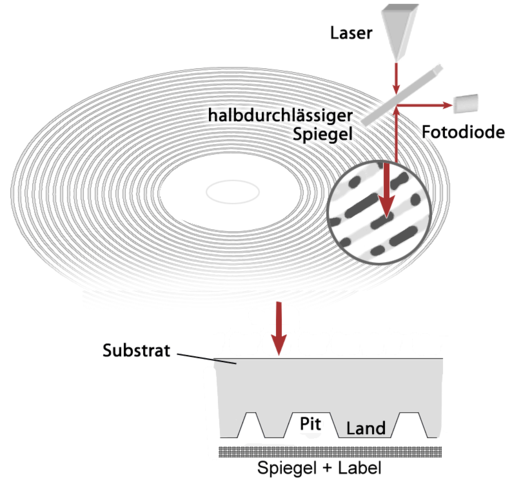
\includegraphics[width=0.6\textwidth]{images/cd} 
				\caption[Funktionsweise optisches Medium \cite{fig:cd}]{Funktionsweise optisches Medium}
				\label{fig:cd}
				\end{figure}
				
        Die allgemeinen Verkaufszahlen von optischen Speichermedien sind in den letzten Jahren gesunken, da nun zunehmen durch h"ohere Bandbreiten des Internets sich neue Distributionswege er"offnet haben.
		

        
{%Gruppe auf   
\label{ch:Technisch:sec:Optische SpeicherungM}     
\begin{table}[ht]
\small
\begin{tabular}{|p{3.8cm}|p{3.2cm}|p{3cm}|p{3cm}|}
\hline
~ & CD & DVD & Blu-ray \\ \hline
Kapazit"at & bis zu 900 MB & 4,7 GB (Single Layer)\newline 8,5 GB (Dual Layer)  & 25 GB (Single Layer) bis zu 500 GB (20 Layer) \\  \hline
Lesegeschwindigkeit & 176 KB/s (CD-DA)\newline 150 KB/s (1x) \newline 10800 KB/s (72x) & 1,385 MB/s (1x) & 36 Mbit/s (8x) \\ \hline
Schreibgeschwindigkeit & 150 KB/s (1x)  8400 KB/s (56x) & 1,385 MB/s (1x) & 4,5 MB/s (1x) (DVD 3x) \\ \hline
Gebrauch & Datenspeicher, Audio-CD & Datenspeicher, Video-DVD & Datenspeicher, Video-Blu-ray \\ \hline
Vorstellung & 1981 & 1995 & 2002 \\
\hline
\end{tabular}
\caption{Vergleich optischer Medien}
\label{tab:vlgOptMed}
\end{table}
}%gruppe zu


        \subsection{CD}
        %% ==============================
        \label{ch:Technisch:sec:Optische Speicherung:sub:CD}
        %% ==============================
        
            Die Compact Disk wurde von Phillips und Sony im Jahr 1981 als Speichermedium f"ur Audio(CD-DA\footnote{Compact Disc - Digital Audio}) eingef"uhrt(vgl. Tabelle \ref{tab:vlgOptMed}). Sp"ater erst wurde die CD als CD-ROM zur Datenspeicherung bei Computer benutzt. 
        
        \subsection{DVD}
        %% ==============================
        \label{ch:Technisch:sec:Optische Speicherung:sub:DVD}
        %% ==============================
        
            Die Digital Versatile Disk\footnote{engl. f"ur digitale vielseitige Scheibe} ist der direkte Nachfolger der CD und wurde mit anwachsenden Speicherbedarf n"otig. 
            \\
            Die h"ohere Speicherkapazit"at bei gleichen Durchmesser kommt durch verschiedene Techniken zu Stande. Zum einen wurden die Strahlen des Abtastlasers gek"uerzt und auch die Wellenl"ange wurde k"urzer. 
			\\
			Der kleine Laserspot erm"oglichte dann feinere Fl"achen abzutasten und somit mehr Informationen pro Fl"acheneinheit zu speichern. Au"serdem wurde im Jahr 2004 die Dual Layer DVD vorgestellt, also die \glqq Doppel-Schichten DVD\grqq{}. Somit konnte man doppelt soviele Daten wie auf einer Single Layer DVD speichern. Bis zu 8,5 Gigabyte waren nun m"oglich.
        
        \subsection{Blu-Ray}
        %% ==============================
        \label{ch:Technisch:sec:Optische Speicherung:sub:Blu-Ray}
        %% ==============================
        
            Die Blu-ray Disc Association stellte 2002 die Blu-ray Disc vor. Der Name zielt auf den Abtastlaser ab, der eine violette Farbe hat. Blu\textbf{e} Ray wurde absichtlich falsch geschrieben, um die Registrierung als Namen zu vereinfachen. Die Blu-ray setzte sich 2008 gegen den Konkurrenten HD-DVD durch und fasst schon mit einem Single Layer 25 Gigabyte. Der Markt f"ur hochaufl"osende Filme war damit f"ur den Endverbraucher ge"offnet.
            \\
           



%%% Local Variables: 
%%% mode: latex
%%% TeX-master: "thesis"
%%% End: 
